\chapter{nD-Laplace}
In this chapter, we delve deeper into geo-indistinguishability and the various mechanisms that work with it.
This is done in the order of the number of dimensions supported by the mechanism:
\begin{enumerate}
  \item 2D-Laplace
  \item 3D-Laplace
  \item nD-Laplace
\end{enumerate}
For each mechanism, we explain the equation for \gls{gi}, the mechanism, and the truncation of data.

%
\newglossaryentry{X}
{
  type=genericmath,
  name={$\ensuremath{X} $},
  description={Set of locations for a user. ($R^2$)},
}
\newglossaryentry{Z}
{
  type=genericmath,
  name={$\ensuremath{Z} $},
  description={For every $x \in X$ a perturbed location $z \in Z$ is reported.},
}
\newglossaryentry{privacy level}
{
  type=genericmath,
  name={$\ensuremath{l} $},
  description={Privacy level},
}
\newglossaryentry{radius}
{
  type=genericmath,
  name={$\ensuremath{r} $},
  description={Radius},
}
\newglossaryentry{Epsilon}
{
  type=genericmath,
  name={$\ensuremath{\epsilon} $},
  description={Defined as $\epsilon = l/r$},
}
\newglossaryentry{theta}
{
  type=genericmath,
  name={$\ensuremath{\theta} $},
  description={Angle},
}

\newpage
\section{2D-Laplace}
The idea of \gls{gi} was introduced to address the issue of privacy and location data \citep{DBLP:journals/corr/abs-1212-1984} (See Equation \ref{algo:2d-geo-indistinguishability}).
It offers an alternative approach for achieving (local) differential privacy for geographical data (latitude/longitude).
The mechanism achieves this by locally adding noise to the location before sending it to a location-based system (LBS).
This section starts with an introduction to mathematics, and for each of the different subsections, we visualize and explain open challenges and theoretic for applying them for clustering.
%\glsaddall
%\leading{10pt}
%\printglossary[type=genericmath, nonumberlist]
%The other symbols can be found in section \ref{section:dp}.
\subsection{Planar and polar Laplace}
In Section \ref{theory:geo-indistinguishability}, we provided an explanation of the concept of \gls{gi}. 
Additionally, we introduced the notion that when a point $x_0 \in X$ serves as the center of a range $r$, a point $z \in Z$ is generated using a noise function \citep{DBLP:journals/corr/abs-1212-1984}. The objective here is to ensure that when the actual locations are $x_0$ and $x_0'$, their divergence is limited to at most $e^{-\epsilon \cdot d(x_0, x_0')}$. This characteristic aligns with the Laplace distribution, which the "planar Laplace" mechanism leverages.
Furthermore, it is worth noting that the "planar Laplace" mechanism is an adaptation of the Laplace distribution designed to accommodate distances in a 2-dimensional space \citep{DBLP:journals/corr/abs-1212-1984}. For clarity, we will refer to this method as "2D-Laplace" from this point forward.

The distance method $d(\cdot, \cdot)$ is a method to calculate the Euclidean distance between two points.
Recalling the definition of Laplace, this method $|x-x'|$ is replaced by the distance metric.
Given the actual location $x_0 \in X$, the \gls{pdf} of the noise mechanism on any other point $z \in Z$ is provided as \citep{DBLP:journals/corr/abs-1212-1984}: 
\begin{equation}
  D_\epsilon(x_0)(z) = \frac{\epsilon^2}{2 \cdot \pi}e^{-\epsilon \cdot d(x_0, z)}
  \label{eq:polar-laplace-pdf}
\end{equation}
The method works for Cartesian coordinates but was modified to support polar coordinates by including $\theta$.
So each polar coordinate is reflected as $(r, \theta)$, where $r = d(x_0, z)$ around point $x_0$.
This idea is visualized in the following figure:
\begin{figure}[H]
  \includesvg[scale=1]{TheorethicalFramework/ND-Laplace/Images/polar-laplace.svg}
  \centering
  \caption{Representation of the generated $(r,\theta)$ and original point $x_0$.}
  \label{figure:parea}
\end{figure}
Next we show in detail, how to generate the polar coordinates $(r, \theta)$. \newline
\textbf{Calculating $r$:}
The $r$ is randomly selected based on a distribution $R$ \citep{DBLP:journals/corr/abs-1212-1984}: 
\begin{equation}
    D_{\epsilon, R}(r) = \int^{2\cdot \pi}_0 \ D_\epsilon(r, \theta) \ d\theta = \epsilon^2 \ r \epsilon^{-\epsilon \cdot r}
    \label{2d:generate-r}
\end{equation}
Where the $r$ is selected randomly on the area of the circle. 
Next, it can be randomly drawn by inverting the \gls{cdf} for the Laplace distribution \citep{DBLP:journals/corr/abs-1212-1984}:
\begin{equation}
  C{_\epsilon}{^{-1}}(p) = - \frac{1}{\epsilon}(W_-1 (\frac{p - 1}{e}) + 1)
  \label{eq:lambert_w_1}
\end{equation}
For this equation, the Lambert $W$ function is used. This function consists of two different branches \citep{corless_lambertw_1996}. This means the value of $W_0(x)$ is always positive, while $W_{-1}(x)$ is always negative. The Lambert w function (also called the product logarithm) is defined as $W(x)e^{W(x)} = x$ \citep{lehtonen_lambert_2016}.
The purpose of the Lambert W function is to invert the \gls{cdf} of the Laplace distribution to generate random noise for one of the coordinates ($r$) using the random value of $p$. It draws the $r$ which will be bounded by the $W_{-1}$, this is very useful for drawing the random planar noise \citep{corless_lambertw_1996}.

\textbf{Calculating $\theta$:}
The other variable ($\theta$) is defined in a similar way \citep{DBLP:journals/corr/abs-1212-1984}: 
\begin{equation}
    D_{\epsilon, \Theta}(\theta) = \int^\infty_0 D_\epsilon(r, \theta) \ dr = \frac{1}{2 \cdot \pi}
    \label{2d:generate-theta}
\end{equation}
To visualize the data, it is necessary to convert the polar coordinates for $(r, \theta)$ to Cartesian coordinates $z = (x, y)$.
This conversion is described as step 4 of the planar Laplace algorithm \citep{DBLP:journals/corr/abs-1212-1984} and visualized using figure \ref{figure:geo}.
\begin{figure}[h]
    \centering
  \includesvg[width=0.8\textwidth]{TheorethicalFramework/ND-Laplace/Images/polar-laplace-to-planar.svg}
  \centering
  \caption{Representation of converting the polar coordinate $(r, \theta)$ to a perturbed point $z = (x, y)$.}
  \label{figure:geo}
\end{figure}

\newpage
\subsection{Truncation} \label{theory:truncation}
After adding the noise to the data, it cannot be ensured the data is within the original domain (figure \ref{figure:truncation-2d}).
If this is not the case, the data is easily distinguished by an unwanted adversary \citep{DBLP:journals/corr/abs-1212-1984,9646489}.
The truncation is an essential part of the mechanism to ensure the data is contained within the domain of the original data $X$. The following example shows two different original points $x_0$ and $x_0'$, where $z$ and $z'$ are being remapped to be within the domain:
%We assume a user has a set of data points with a range of [-1, 1].
\begin{figure}[H]
\centering
  \includesvg[width=1\textwidth]{TheorethicalFramework/ND-Laplace/Images/remapping.svg}
  \caption{Representation of truncation of data points for 2-dimensional Laplace mechanism.}
  \label{figure:truncation-2d}
\end{figure}
%A solution was described by Andres et al. in step 5 of the Laplacian mechanism for 2D space \citep{DBLP:journals/corr/abs-1212-1984}.
%A viable solution is to create a grid around the diameter of the set of points $X = R^2$ that belong to the user \citep{DBLP:journals/corr/abs-1212-1984}.
This approach was introduced by Andres et al. to remap a perturbed point $z$ to the closest point in $G$ \citep{DBLP:journals/corr/abs-1212-1984}.
Here, $G$ is a grid with sides $u$ and $v$, such that $u \leq v$.
%Although this approach remaps data within the original domain of $X$, it is not guaranteed it preserves \gls{gi} anymore.
Let the below equation be the collection of probabilities for a point $z$ being remapped to a closest point in $G$:
\begin{equation}
  R(z) = \{ \ y \in R^2 \ | \ \forall z' \in G \cdot d(y, z') \leq d(y, z') \ \}
  \label{eq:grid-probability}
\end{equation}
The original \gls{gi} definition contains $K$, which is the probability of $z$ being reported as $x_0$ (See Equation: \ref{theory:geo-indistinguishability}).
However, this probability is no longer guaranteed because $z$ can also be part of $G$ \citep{DBLP:journals/corr/abs-1212-1984}.
Hence the probability is now $R(z) = G \cap A$. Where $A$ is a set of acceptable datapoints.\newline
So, $R(z)$ has a different shape depending on the distance $x_0$ and $z$ (ergo, it depends on the grid unit $v$ or $u$). This is due the step units of $G$ stay the same, while the distance $r$ grows \citep{DBLP:journals/corr/abs-1212-1984}.

To overcome this issue, Andres et al. propose a way of calculating $\epsilon'$, depending on the step-unit $u$. \citep{DBLP:journals/corr/abs-1212-1984}.
They proved this and provided theorem 4.1 \citep{DBLP:journals/corr/abs-1212-1984}:
\begin{theorem}[Discretization 2D-Laplace]
  Assume $r_{max} < \frac{u}{\delta_{\theta}}$, and let $q = \frac{u}{r_{max}}\delta_{\theta}$. \\ Let $\epsilon$, $\epsilon' \in R^+$ such that \\
  $\epsilon' + \frac{1}{u}ln \frac{q + 2 e^{\epsilon'u}}{q - 2 e^{\epsilon'u}} \leq \epsilon$ \\
Then $K_{\epsilon'}$ provides $\epsilon$-geo-indistinguishability within the range of $r_{max}$. \\ 
  Namely, if ${d(x_0, z), d(x'_0, z) \leq r_{max}}$ then: \\
  $K_{\epsilon'}(x_0)(z) \leq e^{\epsilon d(x_0, x'_{0})} K_{\epsilon'}(x'_{0})(z)$.
  \label{theorem:discretization}
\end{theorem}
Where $x_0$ and $x_0'$ are two different original points for which the noise is generated. 
Here, $\delta_{\theta}$ is the machine's precision, which is the hardware precision of the GPS-location in the context of geographical data. We will omit this in our research, but still provide the full theorem nonetheless.
The theorem states that $\epsilon'$ is the additional noise needed to satisfy \gls{gi} with the introduction of discretization.
%Then, the final step is truncation based, which is based on the discretization \citep{DBLP:journals/corr/abs-1212-1984}.
It is sufficient to take $r_{max}$ as $diam(A)$, which is the diameter of the set of points $A$ if it satisfies theorem \ref{theorem:discretization} \citep{DBLP:journals/corr/abs-1212-1984}:
So, $r_{max}$ is the maximum distance between points in $A$, which is the area where geo-indistinguishability can be guaranteed \citep{9646489}.
%This idea was later improved by Chatzikokolakis et al., introducing an optimized way of remapping \citep{chatzikokolakis_efficient_2017}.
%The algorithm uses the Bayesian rule to minimize the loss of utility while remapping the data.
%Instead of remapping to the closest point, it remaps to a location where the loss is minimal.
%To decrease the performance impact of this algorithm, it is possible only to consider a specific region around the perturbed point $z$.
%The disadvantage of this method is the need for a prior set of data points to calculate the optimal remapping.
%It does not work for new users and extends the training period.
\subsection{Final mechanism}
Finally, we provide as means of a summary the final algorithm for the Laplace mechanism for 2D space
\begin{algorithm}[H]
  \caption{Full mechanism for perturbing training data for 2D-clustering using planar/2D-Laplace \citep{DBLP:journals/corr/abs-1212-1984}}\label{alg:rq1}
  \begin{algorithmic}
    \Require $x \in X$  \Comment 2D array of points \\
    $\epsilon$ \Comment should satisfy Theorem \ref{theorem:discretization}
    \Ensure $z \in Z$ \Comment 2D array of perturbed points
    %\State $r = \frac{\sigma}{2}$ \Comment formula 4.1
    %\State $\epsilon = \frac{l}{r}$ \Comment Calculating privacy budget \citep{DBLP:journals/corr/abs-1212-1984}
    \State $x_{min} \gets min(X)$
    \State $x_{max} \gets max(X)$
    \State $Z \gets []$
    \For{$point_i \in X$}
    \State $\theta \gets [0, \pi2]$       \Comment Random noise for $\theta$
    \State $p \gets [0, 1]$
    \State $z_i \gets C{_\epsilon}{^{-1}}(p)$       \Comment formula 3.2
    %\State $z_i \gets T(x_{min}, x_{max}, point_i, z_i)$ \Comment algorithm 1.
    \State $x_{perturbed} \gets point_{i_x} + (z_{i_x} * \cos(\theta)) $ \Comment add noise to x-coordinate
    \State $y_{perturbed} \gets point_{i_y} + (z_{i_y} * \sin(\theta)) $ \Comment add noise to y-coordinate
    \State append $x_{perturbed}, y_{perturbed}$ to Z
    \EndFor
    \State \Return Z
  \end{algorithmic}
  \label{alg:2d-laplace}
\end{algorithm}
\newpage
\section{3D-Laplace}
\todo[inline]{Is considered for research question 3}

\newpage
\section{nD-Laplace}
As mentioned in the previous chapter, the paper that was introduced by Min et al. is be-able to handle 3-dimensional data.
A small recap: a point $(r, \theta, \psi)$ gives us the spherical coordinates of a given 3-dimensional sphere.
An important property for this is the fact that each of these coordinates can be generated separately \citep{DBLP:journals/corr/abs-1212-1984, 9646489}.
The $r$ gives us the radius or distance from $(\theta, \psi)$ to the center of the sphere \footnote{https://mathworld.wolfram.com/SphericalCoordinates.html}.
So, instead of having just these two coordinates, we are be-able to extend this to n-dimensions by considering an n-hypersphere \citep{fernandes_generalised_2019, 9646489}.
To this end, besides points $\theta$ and $\psi$ we also consider $\theta \in S^n$, where S is a unit hypersphere.

The first step to generate the noise is first to select the $r$.
This method is almost identical to the one for 3-dimensional (\ref{eq:3d-laplace-r}).
But, instead of applying a scale of 3, the scale will be $n$ for the number of dimensions in the data \citep{fernandes_generalised_2019}:
\begin{equation}
  \gamma(n, 1/\epsilon)
\end{equation}
For the other dimensions, we consider a vector $U = (\theta_1, \theta_2, \theta_n)$ which is uniformly selected based on a unit $n$-hypersphere $S^n$ \citep{fernandes_generalised_2019}.
We consider the work that was proposed by Marsaglia et al. for 4-sphere that can be used for selecting points from an n-hypersphere \citep{marsaglia_choosing_1972}.
This method resolves around selecting points from a hypersphere by using a uniform distribution for the domain [0, 1].
We adopted the approach that uses the Gaussian distribution \footnote{https://mathworld.wolfram.com/SpherePointPicking.html}.

\subsection{Cartesian coordinates}
As with the 2/3D-Laplace, the spherical coordinates need to be converted to Cartesian to be able to cluster.
It is comparable to the way it was done in the previous chapters, however, as there are an $n$-amount of angles the equation is repeated and slightly different:
\begin{align*}
  x_1 = r * cos (\theta_1)                                          \\
  x_2 = r * sin (\theta_1) * cos (\theta_2)                         \\
  x_{n} = r * sin(\theta_1) … sin(\theta_{n-2}) *cos (\theta_{n-1}) \\
  x_n = r * sin(\theta_{n-1}) * sin(\theta_{n-2}) * sin(\theta_{n-1})
\end{align*}
If we combine sections 1 and 2 of this chapter, we are being able to give a good overview of the solution using a similar image as for the 2D and 3D variants (figure \ref{fig:nd-laplace-overview}).
\begin{figure}[ht]
  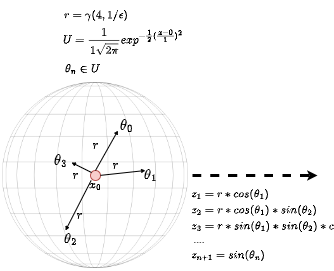
\includegraphics[width=0.6\textwidth]{TheorethicalFramework/ND-Laplace/Images/nd_laplace.png}
  \caption{Overview of the nD-Laplace mechanism}
  \label{fig:nd-laplace-overview}
\end{figure}
\newpage
\subsection{Privacy versus utility} \label{theory:privacy-utility-nd}
If we continue adding dimensions, we notice the noise is shrinking proportionally.
To understand this behavior, we first have to examine the formula for a hypersphere’s volume.
\begin{equation}
  S_n = \frac{2 \pi^{n/2}}{\gamma(\frac{1}{2}n)}
\end{equation}
Where $\gamma$ is the gamma distribution that is determined based on the number of dimensions $n$ \footnote{https://mathworld.wolfram.com/Hypersphere.html}.
As the amount of dimensions increases, the most volume is located on the hypersphere surface.
When we convert the points to Cartesian coordinates, some will be located at the center (e.g., 0.5), while others will be close to the surface (e.g., 0.0).
However, as the number of dimensions increases, the majority will be close to the surface (e.g., 0.99).
The decreasing amount of volume is illustrated using this figure:
\begin{figure}[H]
  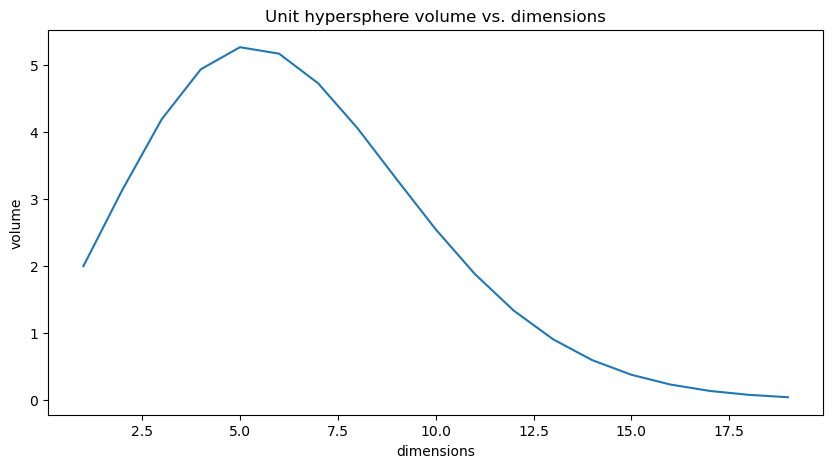
\includegraphics[width=0.8\textwidth]{TheorethicalFramework/ND-Laplace/Images/volume.png}
  \caption{Illustration of the decreasing volume while increasing the number of dimensions}
  \label{fig:curse-of-dimensionality}
\end{figure}

The noise decreases as the dimensions increase, increasing utility.
Hence, it is intriguing to observe the behavior of privacy relative to utility.
This behavior will be further emphasized in a later stage of this research.
\newpage
\subsection{Truncation}
For 2D/3D Laplace, a grid and cuboid were respectively introduced to truncate noise mechanisms \citep{DBLP:journals/corr/abs-1212-1984,9646489}.
This section extends the work done for 2D and 3D Laplace (\ref{theory:truncation}, \ref{2d:optimizing}) \newline
This section introduces an extension for handling any number of dimensions, which can also substitute for 2D/3D.
We want to note that this section focuses on improving utility with remapping.
Any remap function preserves geo-indistinguishability \cite{chatzikokolakis_efficient_2017}, so the required privacy is still preserved.

Recalling both mechanisms, the 2D version operates on a plane and approximates on a grid $G$, while the 3D version works in a 3D space using a cuboid grid.
Given a set of input points $X \subset R^2$, we can truncate points that are outside the domain by remapping them to points within $G$ ($Z = X \cap G$) \citep{DBLP:journals/corr/abs-1212-1984}.
Here, $X$ represents other data points reported locally by the same user.
To extend this approach to n-dimensional data, we need an efficient way to search points in an n-dimensional hypersphere.
To do this, we adopt the idea proposed by Chatzikokolakis et al. of using a kd-tree for efficient searching of the grid \citep{chatzikokolakis_efficient_2017}.
In their research, they describe the utilization of a kd-tree for searching nearby points for a given point.
For this reason, we also use a kd-tree for the following tasks:
\begin{enumerate}
  \item Finding nearby points for $z \in G$ (section: \hyperref[theory:grid-remapping]{Grid with kd-tree remapping}).
  \item Finding nearby points for $x \in X$ and $z \in Z$ (section \hyperref[theory:optimal-remapping]{Optimal remapping}).
\end{enumerate}
For visualization purposes, this section will primarily focus on 2D data.
However, it is important to emphasize that the same algorithm will also be applied to 3D and nD data. The underlying principles and steps of the algorithm remain the same.

We first give an introduction to kd-trees on the next page and then explain how we apply them for the two tasks.

\newpage
\subsubsection*{Kd-trees} \label{theory:kd-trees}
A kd-tree is a algorithm that can be used to search a grid for nearby points \citep{bentley_multidimensional_1975}.
It is capable of doing so, by recursively splitting the grid into a binary tree to search for grid coordinates \citep{washington_k-d_2002}.
In addition to this, it preserves spatial information of the data so it can be utilised to find nearby points using Euclidean distance (nearest neighbor search).
The following example provides an idea on how this works (Figure \ref{fig:kd-tree-theory}):
\begin{figure}[H]
  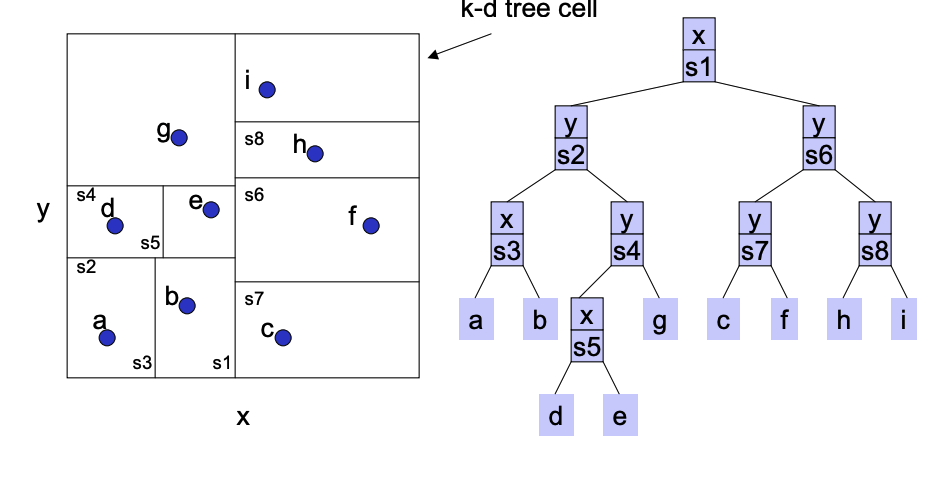
\includegraphics[width=0.8\textwidth]{TheorethicalFramework/ND-Laplace/Images/kd-tree-part1.png}
  \caption{Representation of constructing a kd-tree with 2 dimensions \citep{washington_k-d_2002}.}
  \label{fig:kd-tree-theory}
\end{figure}
Take, for example, the 2D Laplace algorithm that utilizes a plane (left side).
The data points can be divided based on their x and y coordinates.
Each coordinate becomes a node in the binary tree, and the grid is divided based on these splits.
The binary tree allows us to efficiently search the grid. An expample of this is provided in the following image (Figure \ref{fig:kd-tree-searching-theory}):
\begin{figure}[H]
  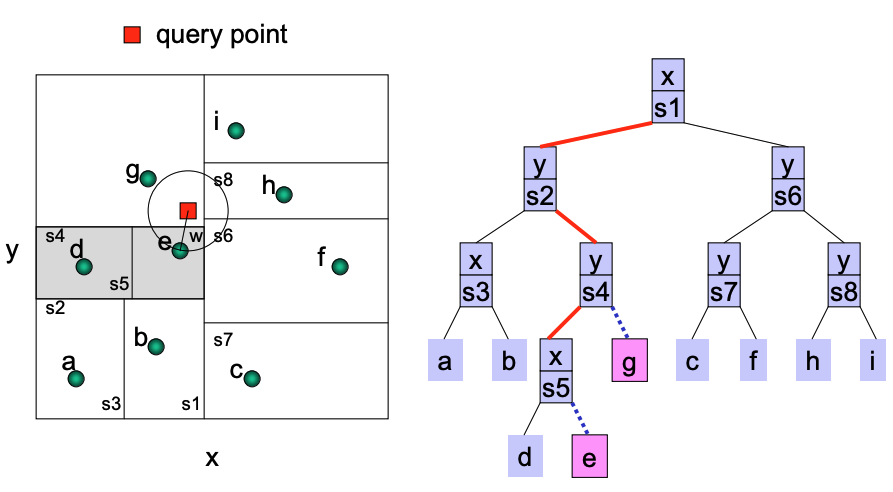
\includegraphics[width=0.8\textwidth]{TheorethicalFramework/ND-Laplace/Images/kd-tree-part2.png}
  \caption{Representation of a searching a kd-tree with 2 dimensions \citep{washington_k-d_2002}.}
  \label{fig:kd-tree-searching-theory}
\end{figure}
In the example, we are searching for all points that fall within the radius of a random query point.
Thanks to the grid being divided into a binary tree, a portion of the grid can be efficiently searched, evaluated and referenced.
The biggest advantage is that this greatly reduces the complexity of searching.
Constructing the kd-tree only costs $O(kn)$, where $k$ is the number of dimensions and $n$ is the dataset size.
Searching for a nearest neighbor is a little less efficient, with a time complexity of $O(\log n)$ \citep{washington_k-d_2002}.
A reference to the Big O notation can be found in the attachment \todo{add reference}.
\subsubsection{Grid with kd-tree remapping} \label{theory:grid-remapping}
As explained in the previous paragraph, a kd-tree can be used to perform a nearest neighbor search.
This is highly relevant to our research as it proves to be beneficial for the optimizations we are striving for.
To this end, we adopt this approach for remapping the perturbed datapoints $z \in Z$ to a grid $G$. \newline
We have illustrated the three steps required for this below:
\begin{figure}[H]
  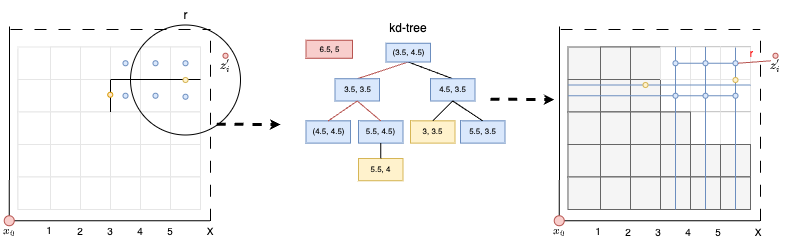
\includegraphics[width=1\textwidth]{TheorethicalFramework/ND-Laplace/Images/KD-tree.png}
  \caption{Representation of a kd-tree with 2 dimensions to remap based on a grid.}
  \label{fig:kd-tree}
\end{figure}
%When using a kd-tree to search for a data point $z_i$, the algorithm begins with an unbalanced binary tree.
%The root is split by the x-axis, and since 4.5 is greater than 3.5, we go to the right.
%This means that we no longer need to consider the left (greyed out) part of the grid.
%We continue traversing the tree until we find the nearest point based on Euclidean distance.
The above illustration presents the grid-remapping algoritm.
Firstly, a grid is generated, where each (blue) point represents the center of a grid cell.
Together, these centroids form the grid dataset, denoted as $G$.
The yellow points and $x_i$ are part of the original collection, denoted as $X$.
Here, $r$ represents the radius used to generate a private version of the data point $x_i$, named $z_i$, based on 2D-Laplace (in this case).
In the illustration, you can observe that $z_i$ falls outside the original domain of $X$, and for this reason, it needs to be remapped.
We accomplish this by utilizing the nearest-neighbor search from the kd-tree algorithm, allowing us to search in $X \cup G$.
Using this algorithm, we can effectively remap point $z \in Z$ to either $X$ or $G$ based on the closest Euclidean distance (Algorithm \ref{alg:grid-remapping-laplace} and Algorithm \ref{alg:find-outside-domain-laplace}).

The utility of this method depends on the number of grid cells in $G$, since a smaller distance will result in more frequent mapping to the surface of the grid.
When $\epsilon$ is very low (and thus farther away), the data points are more likely to map to the grid surface (\ref{fig:3d-laplace-noise}, \ref{fig:3d-laplace-example}).
Increasing the number of grid cells can improve the utility, but this comes at the cost of significantly increased space complexity for $k$ dimensions.
This is because a grid of $n*m$ dimensions has a complexity of $O(n^2)$.
Therefore, we also explore the optimal remapping algorithm proposed by Chatzikokolakis et al \citep{chatzikokolakis_efficient_2017}.
\begin{algorithm}[H]
  \caption{Algorithm for finding points outside the domain of $X$.}
  \begin{algorithmic}
    \Require $x \in X$  
    \Require $z \in Z$ 
    %\State $tree \gets KDTree(X)$ \Comment construct a KDTree from the original data.
    \State $X_{domain} \gets \Call{KDTree::query}{Z}$ \Comment find the closest points.
    \State $X_{features} \gets \Call{List::getfeatures}{X}$ 
    \State $X_{outside-domain} \gets []$
    \For{$feature \in X_{features}$} 
    \If{$feature \leq \Call{X::min}{Z} $}
    \State $\Call{row::append}{X_{outside-domain}}$
    \EndIf
    \If{$feature \geq \Call{X::max}{Z} $}
    \State $\Call{row::append}{X_{outside-domain}}$
    \EndIf
    \EndFor
    \State \Return $X_{outside-domain}$ 
  \end{algorithmic}
  \label{alg:find-outside-domain-laplace}
\end{algorithm}
\begin{algorithm}[H]
  \caption{Algorithm for generating and remapping to a grid.}
  \begin{algorithmic}
    \Require $x \in X$  \Comment original dataset
    \Require $z \in Z$ \Comment perturbed dataset
    \Require $grid$ \Comment grid structure ($n * m$)
    %\State $tree \gets KDTree(X)$ \Comment construct a KDTree from the original data.
    %\State $X_{domain} \gets$ \Call{KDTree::query}{$Z$} \Comment find the closest points.
    \State $d_{X} = dist(Z, X)$ \Comment euclidean distances
    \State $d_{grid} = dist(Z, grid)$ 
    \State $Z_{out-domain} \gets FindPointsOutsideDomainX(X, Z)$ \Comment Algorithm \ref{alg:find-outside-domain-laplace}
    \State $grid_{tree} \gets KDTree(grid)$ 
    \State $grid_{mask} \gets KDTree::query(Z)$ \Comment find indices of $z \in Z$ that are closeby grid cells.
    \State $Z_{grid-mask} \gets Z_{out-domain} \cup d_{grid} < d_{X}$ \Comment All points $z \in Z$ that are closeby grid cells and are outside domain.
    \State $Z` \gets Z[grid[grid_{mask}][Z_{grid-mask}]]$ \Comment combinate masks to set appropiate indexes to $g \in grid$.
    \State \Return $Z`$
  \end{algorithmic}
  \label{alg:grid-remapping-laplace}
\end{algorithm}
\newpage
\subsubsection{Optimal remapping} \label{theory:optimal-remapping}
As we discussed, the remapping will be performance intensive to be-able to provide good utility and that is why we adopt the optimal remapping \citep{chatzikokolakis_efficient_2017}.
Consider the grid that was proposed in \ref{fig:kd-tree}.
After remapping point $z_i$, it is mapped to the center for the grid cell.
Based on the cell width, the distance to the original point $x_i$ and $ z_i$ could be really large.
Our goal is to remap the center of the grid cell (now $z_i$) to a point that is closer to $x_i$ (if applicable). \newline
This is visualized by zooming into the last step of the grid-remapping (Figure \ref{fig:kd-tree}).
\begin{figure}[H]
  %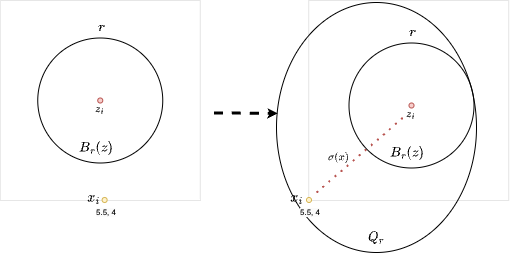
\includegraphics[width=0.7\textwidth]{TheorethicalFramework/ND-Laplace/Images/optimal-remapping.png}
  \includesvg[width=1\textwidth]{TheorethicalFramework/ND-Laplace/Images/optimal-remapping}
  \caption{Representation of optimal remapping \citep{chatzikokolakis_efficient_2017}, where $z_i$ is remapped to $x_i$ using $\sigma(x)$ instead of the center of the grid cell.}
  \label{fig:optimal-remapping}
\end{figure}
In Figure \ref{fig:optimal-remapping} we can observe that $z_i$ is remapped to the center of the grid cell as a consequence of the grid-remapping.
For the reasons mentioned earlier, this is not optimal, and we can further optimize it by utilizing the other data points.
The remapping algorithm works on the idea of crowded places \ref{2d:optimizing}, with the intuition that a crowded place leverages indistinguishability by crowdedness \citep{chatzikokolakis_efficient_2017}.
For the remainder of this thesis, we will use the term "density" instead of "crowdedness" because it better aligns with the clustering of data.

The first step is to calculate $B_r(z)$, which refers to all the data points that fall within the original radius $r$ around the data point $z_i$.
The next step in the algorithm is to collect the data points around $x_i$, in order to calculate how closely it can be remapped to $z_i$ while preserving distinguishability.
This is the collection (convex hull) of all original data points $x \in X$ that are close to $x_i$, determined based on the radius $r$ around $x_i$.
Finally, we combine both sets to obtain $Q_r = B_r \cap X$.
Now that we have the sets of points around $x_i$ and $z_i$, we can calculate the density for each point $q \in Q_r$ \citep{chatzikokolakis_efficient_2017}:
\begin{equation}
  \forall x \in Q_r \quad \sigma(x) = \frac{w(x)e^{-\epsilon d(x, z)}}{\sum{_{q\in Q_r} w(q)e^{-\epsilon d(q, z)}}}
  \label{eq:optimal-remapping-formula-1}
\end{equation}
Where $w(q)$ is the weight of a point $q in Q_r$, and can be seen as points that are visited earlier by the user or other users (e.g. point of interests).
We will revisit this topic in the next paragraph when discussing the practical implementation of the nd-Laplace algorithm.
The same applies to $w(x)$, but for an individual point $q \in Q_r$ instead of the summation.
Finally, the new $z'$ is calculated by taking the mean value of $\sigma(x)$ \citep{chatzikokolakis_efficient_2017}.
\todo{Also include equations for generating coefficinets and probabilities}
%Chatzikokolakis et al's work considers a prior set of data point $Q \in R^n$.
%Which are other data points that belong to the user.
%We are interested in the data points that are within the radius $r$ around $z$.
%This is denoted as $B_r(z)$, which is the vector of all points within radius $r$ around $z$.
%In addition to this, there is also a $Q_r$ that is a convex hull of all nearby points.
%Hence, this is described as $Q_r = B_r \cap Q$.
%The final intuition here is that $r$ is automatically generated based on crowdedness (see circle inside figure \ref{fig:optimal-remapping}).
%The last step is to take the mean value of $\sigma(x)$.
%Unfortunately, optimal remapping is not possible for users that do not have sufficient data (e.g. new users).
%The remapping is not applied for these users and is also not applied for $z$ if it is within the domain of $X$.
\subsubsection{Practical implementation}
It is difficult to interpret $w(q) \in Q_r$ beforehand based on other users, as we do not have this information (there is a way, but we explain this at the end of this section).
To this end, we will interpret $w(x)$ as the number of points within the radius $r$ around a point $x \in Q_r$.
Afterwards, it is possible to divide the outcome of this value by the sum of these points (as done in Algorithm \ref{eq:optimal-remapping-formula-1}).
We therefore remain to the same algoritm as proposed by Chatzikokolakis et al. but interpret the weight differently.

It is however still possible to interpret $w(q)$ as the weight based on other user's datapoints.
This requires us to implement the mechanism interactively.
In this approach, all clients perturb their data and sent it to the server.
The server clusters the private data and calculates weight based on cluster information (e.g., crowdedness/density) and shares it with the clients.
The clients then use the optimal remap and share their private information with the server again.
Although this system requires only a single round-trip between server and clients, it reveals cluster information, so we prefer the non-interactive setup.

\begin{algorithm}[H]
  \caption{Algorithm to implement the density remapping of $z \in Z$ to be in the domain of $x \in X$}
  \begin{algorithmic}[1]
    \Require $x \in X$
    \Require $z \in Z$
    \Require $epsilon$
    \Ensure $z' \in Z$
    \State $Z' = FindRemappedPoints(Z)$ \Comment Algorithm: \ref{alg:find-outside-domain-laplace}
    \State $tree \gets KDTree(X)$
    \For{$z' \in Z'$}
    \State $r = \Call{FindRadius}{(z')}$ \Comment Get original radius $r$.
    \State $X_r \gets \Call{KDTree::query}{x}$ \Comment find $q \in X$ around $x$ with radius $r$.
    \State $B_r \gets \Call{KDTree::query}{z'} $
    \State $\sigma(x) = []$
    \State $Q_r = \gets X_r \cap B_r$
    \State $w_x = \Call{Length}{X_r, B_r}$ \Comment weight is simply adding density of $X_r$ and $B_r$.
    \For{$q \in Q_r$}
    \State $q \gets \Call{KDTree::query}{q}$
    \State $w_q = \Call{Length}{Q_r}$ \Comment $w_q$ is the density of each point $q$ within $Q_r$.
    \State $\sigma(w_x) \gets \Call{Remap}{w_x, \epsilon}$ \Comment Equation \ref{eq:optimal-remapping-formula-1}.
    \State $\sigma(x) \gets \Call{Append}{\sigma}$ \Comment add to the list $\sigma(x)$.
    \EndFor
    \State $z' \gets \Call{Average}{\sigma(x)}$ \Comment Equation: \ref{eq:optimal-remapping-formula-2}.
    \EndFor
  \end{algorithmic}
  \label{alg:optimal-remapping-laplace}
\end{algorithm}

\begin{itemize}
  \item 1: Receives all the points $z \in Z$ that are outside the domain of $X$.
  \item 2: Constructs a KDTree from the original data $X$, so it can be queried.
  \item 3: Receives the original privacy radius $r$ that was used to generate $z$ from $x$.
  \item 4: $X_r$ is the set of points $x \in X$ that are within the radius $r$ of $x$.
  \item 5: $B_r$ is the set of points $z \in Z$ that are within the radius $r$ of $z$.
  \item 7: $w_x$ is the "popularity" of $x$ and $z$, for the number of points is counted within the radius $r$.
  \item 12: $w_q$ is the weight of each point $q \in Q_r$, so $q$ is re-assigned to be the number of points within the radius $r$ of $q$.
\end{itemize}

\newpage
The equation for density remapping \ref{eq:optimal-remapping-formula-1} was created for 2-dimensional data.
However, we aim to use this same approach for 3-dimensional and n-dimensional data.
To do so, we first revisit the \gls{pdf} for 3D-Laplace, which was defined using this Equation: \ref{eq:3d-laplace-pdf}.
Few modifications are necessary, as the normalization factor $A$ is now defined using Equation: \ref{eq:optimal-remapping-formula-1}.
\todo[inline]{Formulate the definition of $A$}
\todo[inline]{Check if this can be extended to nD-Laplace}


\subsection{Putting it together}
\todo[inline]{Create algorithm for nD-Laplace}
\begin{algorithm}[H]
    \caption{Full algorithm for perturbing training data for nD-clustering using planar/2D-Laplace \citep{DBLP:journals/corr/abs-1212-1984}}\label{alg:rq1}
    \begin{algorithmic}
      \Require $x \in X$  \Comment 2D array of points
      \Require $l \in R^ +$
      
      \State \Return Z
    \end{algorithmic}
    \label{alg:nd-laplace}
  \end{algorithm}
%\subsection{Extending to $d_x$-privacy}
%\todo[inline]{Find if this is possible}

%Constructing elastic distinguishability metrics for location privacy
\newpage

\subsection{Mechanism flowchart}
All formulas and theories are established for 2D, 3D, and nD-Laplace, so the mechanism design applies to all three variants:
\begin{figure}[h]
  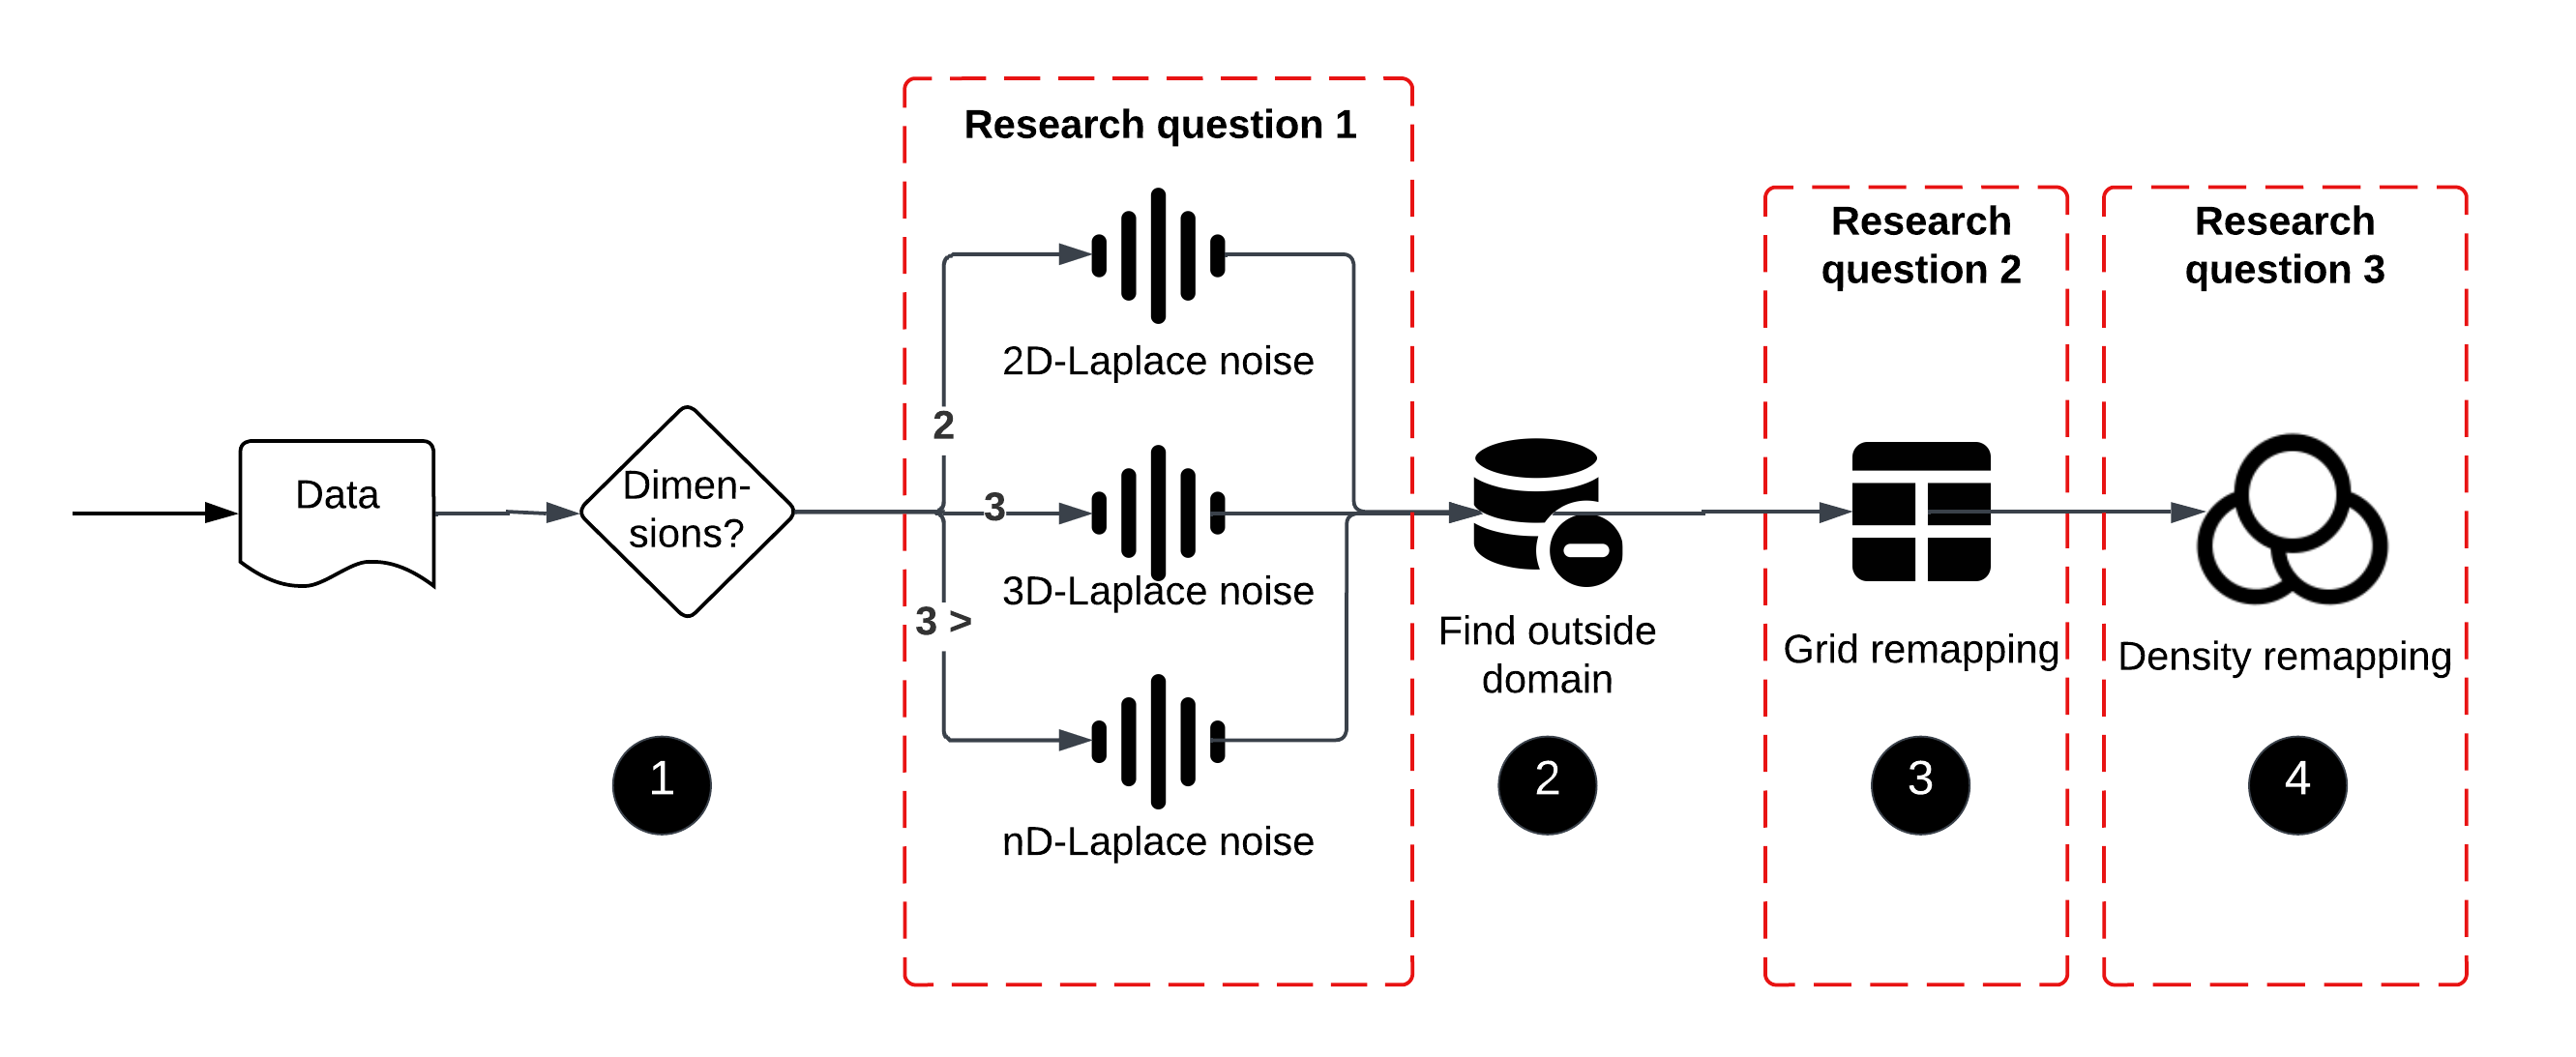
\includegraphics[width=1.1\textwidth]{TheorethicalFramework//ND-Laplace//Images/Thesis-nd - final-mechanism-design.png}
  \caption{Non-interactive mechanism design for nD-Laplace.}
  \label{fig:final-mechanism-design}
\end{figure}
%\todo[inline]{Modify to density-nD-Laplace \& nD-Laplace for image reporting}
For easy navigation, we provide a list of all algorithms:
\begin{enumerate}
  \item Based on the number of dimensions, the algorithm decides the correct Laplace mechanism to use:
        \begin{itemize}
          \item 2D-Laplace:  \ref{alg:2d-laplace}
          \item 3D-Laplace: \ref{alg:3d-laplace}
          \item nD-Laplace: \ref{alg:nd-laplace}
        \end{itemize}
  \item Find points outside domain: \ref{alg:find-outside-domain-laplace}
  \item Grid remapping: \ref{alg:grid-remapping-laplace}
  \item Density remapping: \ref{alg:optimal-remapping-laplace}
\end{enumerate}
\added{In addition, relevant research questions are incorporated into the architecture overview.
These questions are covered in chapter \ref{chapter:methodology}}.
\subsubsection{Practical example}
The shape of the dataset is necessary for the usefulness of clustering.
With our algorithm, there are four different shapes/variants of the dataset.
For example, this has been visualized using a 3D dataset based on the heart dataset (\ref{datasets-section}).
Our mechanism aims to provide privacy and preserve the dataset's shape to benefit the utility of clustering.
Grid remapping and optimal remapping are used to achieve this goal.

\begin{figure}[H]
  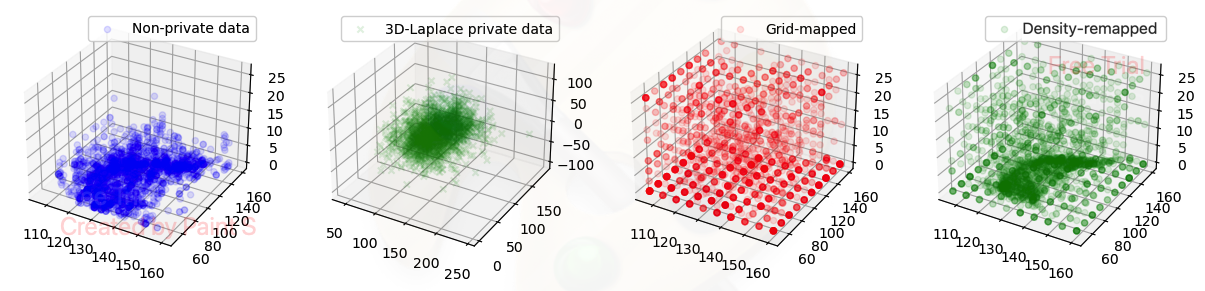
\includegraphics[width=1.1\textwidth]{TheorethicalFramework/ND-Laplace/Images/optimal-remapping-example.png}
  \caption{Example of optimal remapping for the 3D-dataset: Cardiotocography. The example shows the different steps of the mechanism in sequence for a dataset perturbed with a privacy budget of 0.1.}
\end{figure}

\begin{enumerate}
  \item Dataset: the blue dots represent the original dataset without any modifications.
  \item Adding noise: the green crosses represent the dataset after adding noise; for this particular example, this is 3D-Laplace (Algorithm \ref{alg:3d-laplace}):
        As can be observed, the data is generated from the center, causing many data points to fall outside the original domain of the dataset.
  \item Grid-remapping: the red dots represent the dataset after grid-remapping (Algorithm \ref{alg:grid-remapping-laplace})
        After performing the grid remapping algorithm, all points within the domain are plotted.
        However, the original shape of the data is mostly lost.
        This makes it challenging to cluster the data as was possible with the original data.
  \item Optimal-remapping: the green dots represent the dataset after optimal-remapping (Algorithm \ref{alg:optimal-remapping-laplace}).
        After completing the previous step, the data points are again remapped based on the (original) density.
        This results in restoring the original shape of the data and, consequently, the clusters.
\end{enumerate}

